{\heiti 第八章~习题}

1. 证明对于六角密堆积结构,理想的$c/a$比是$\bigg(\dfrac83\bigg)^{1/2}\approx1.633$

证明:~六角密堆积是ABAB堆积,其格子是六角\textrm{Bravais}格子,当两个直径相等的刚性球密堆积时即为理想的密堆积。如图\ref{Fig:Hexagonal_closed-packed_structure}所示\\
\begin{figure}[h!]
\centering
\vspace*{-0.05in}
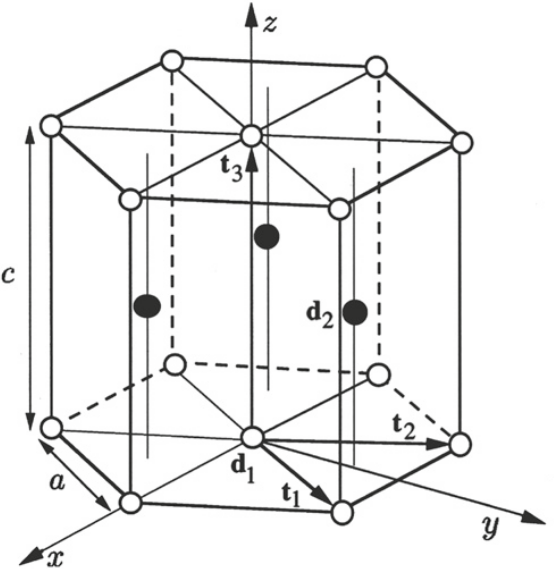
\includegraphics[height=1.65in,width=1.65in,viewport=0 0 554 569,clip]{Figures/Hexagonal_closed-packed_structure.png}
\caption{\small \textrm{理想六方密堆积平移基矢$\vec t_1$、$t_2$、$t_3$及两个原子位置$\vec d_1$、$d_2$示意图.}}%(与文献\cite{EPJB33-47_2003}图1对比)
\label{Fig:Hexagonal_closed-packed_structure}
\end{figure}
不难看出,基矢可用$a$和$c$表示为:~$\vec t_1=a(\frac12,\frac{\sqrt 3}2,0)$,$\vec t_2=a(-\frac12,\frac{\sqrt 3}2,0)$,$\vec t_1=c(0,0,1)$\\
类似地,原子位置可表示$\vec d_1=(0,0,0)$,$\vec d_2=(0,\frac{a}{\sqrt 3},\frac{c}2)$\\
设刚性球半径为$r_0$,据密堆积条件有等量关系
\begin{displaymath}
	\begin{aligned}
		2r_0=&a\\
		|d_2|=&\sqrt{(a^2/3)+(c^2/4)}=2r_0
	\end{aligned}
\end{displaymath}
故
\begin{displaymath}
	\begin{aligned}
		a^2=&a^2/3+c^2/4\\
		8a^2&=3c^2\\
		\therefore~c/a=&\bigg(\dfrac83\bigg)^{1/2}\approx1.633
	\end{aligned}
\end{displaymath}
得证

2. 证明:~体心立方晶格的倒格子是面心立方;~面芯立方晶格的倒格子是体心立方
证明:~根据倒格子的定义
\begin{displaymath}
	\begin{aligned}
		\vec b_1=&2\pi\dfrac{\vec a_2\times\vec a_3}{\vec a_1\cdot(\vec a_2\times\vec a_3)}\\
		\vec b_2=&2\pi\dfrac{\vec a_3\times\vec a_1}{\vec a_1\cdot(\vec a_2\times\vec a_3)}\\
		\vec b_3=&2\pi\dfrac{\vec a_1\times\vec a_2}{\vec a_1\cdot(\vec a_2\times\vec a_3)}
	\end{aligned}
\end{displaymath}
(1)~体心立方格子原胞的基矢
\begin{displaymath}
	\begin{aligned}
		\vec a_1=&\dfrac{a}2(-\mathbf{i}+\mathbf{j}+\mathbf{k})\\
		\vec a_2=&\dfrac{a}2(\mathbf{i}-\mathbf{j}+\mathbf{k})\\
		\vec a_1=&\dfrac{a}2(\mathbf{i}+\mathbf{j}-\mathbf{k})\\
	\end{aligned}
\end{displaymath}
因此有倒格子基矢为
\begin{displaymath}
	\begin{aligned}
		\vec b_1=&2\pi\dfrac{\vec a_2\times\vec a_3}{\vec a_1\cdot(\vec a_2\times\vec a_3)}=\dfrac{2\pi}{v_0}\dfrac{a}2(\mathbf{i}-\mathbf{j}+\mathbf{k})\times\dfrac{a}2(\mathbf{i}+\mathbf{j}-\mathbf{k})\\
		=&\dfrac{2\pi}{v_0}\dfrac{a^2}4(\mathbf{i}-\mathbf{j}+\mathbf{k})\times(\mathbf{i}+\mathbf{j}-\mathbf{k})=\dfrac{2\pi}a(\mathbf{j}+\mathbf{k})\\
		\vec b_2=&2\pi\dfrac{\vec a_3\times\vec a_1}{\vec a_1\cdot(\vec a_2\times\vec a_3)}=\dfrac{2\pi}{v_0}\dfrac{a}2(\mathbf{i}+\mathbf{j}-\mathbf{k})\times\dfrac{a}2(-\mathbf{i}+\mathbf{j}+\mathbf{k})\\
		=&\dfrac{2\pi}{v_0}\dfrac{a^2}4(\mathbf{i}+\mathbf{j}-\mathbf{k})\times(-\mathbf{i}+\mathbf{j}+\mathbf{k})=\dfrac{2\pi}a(\mathbf{k}+\mathbf{i})\\
		\vec b_3=&2\pi\dfrac{\vec a_1\times\vec a_2}{\vec a_1\cdot(\vec a_2\times\vec a_3)}=\dfrac{2\pi}{v_0}\dfrac{a}2(-\mathbf{i}+\mathbf{j}+\mathbf{k})\times\dfrac{a}2(\mathbf{i}-\mathbf{j}+\mathbf{k})\\
		=&\dfrac{2\pi}{v_0}\dfrac{a^2}4(-\mathbf{i}+\mathbf{j}+\mathbf{k})\times(\mathbf{i}-\mathbf{j}+\mathbf{k})=\dfrac{2\pi}a(\mathbf{i}+\mathbf{j})
	\end{aligned}
\end{displaymath}
因此$\vec b_1$,$\vec b_2$,$\vec b_3$为基矢构成的格子是面心立方格子

(2)~面心立方格子原胞的基矢
\begin{displaymath}
	\begin{aligned}
		\vec a_1=&\dfrac{a}2(\mathbf{j}+\mathbf{k})\\
		\vec a_2=&\dfrac{a}2(\mathbf{k}+\mathbf{i})\\
		\vec a_1=&\dfrac{a}2(\mathbf{i}+\mathbf{j})\\
	\end{aligned}
\end{displaymath}
因此有倒格子基矢为
\begin{displaymath}
	\begin{aligned}
		\vec b_1=&2\pi\dfrac{\vec a_2\times\vec a_3}{\vec a_1\cdot(\vec a_2\times\vec a_3)}=\dfrac{2\pi}{v_0}\dfrac{a}2(\mathbf{k}+\mathbf{i})\times\dfrac{a}2(\mathbf{i}+\mathbf{j})\\
		=&\dfrac{2\pi}{v_0}\dfrac{a^2}4(\mathbf{k}+\mathbf{i})\times(\mathbf{i}+\mathbf{j})=\dfrac{2\pi}a(-\mathbf{i}+\mathbf{j}+\mathbf{k})\\
		\vec b_2=&2\pi\dfrac{\vec a_3\times\vec a_1}{\vec a_1\cdot(\vec a_2\times\vec a_3)}=\dfrac{2\pi}{v_0}\dfrac{a}2(\mathbf{i}+\mathbf{j})\times\dfrac{a}2(\mathbf{j}+\mathbf{k})\\
		=&\dfrac{2\pi}{v_0}\dfrac{a^2}4(\mathbf{i}+\mathbf{j})\times(\mathbf{j}+\mathbf{k})=\dfrac{2\pi}a(\mathbf{i}-\mathbf{j}+\mathbf{k})\\
		\vec b_3=&2\pi\dfrac{\vec a_1\times\vec a_2}{\vec a_1\cdot(\vec a_2\times\vec a_3)}=\dfrac{2\pi}{v_0}\dfrac{a}2(\mathbf{j}+\mathbf{k})\times\dfrac{a}2(\mathbf{k}+\mathbf{i})\\
		=&\dfrac{2\pi}{v_0}\dfrac{a^2}4(\mathbf{j}+\mathbf{k})\times(\mathbf{k}+\mathbf{i})=\dfrac{2\pi}a(\mathbf{i}+\mathbf{j}-\mathbf{k})
	\end{aligned}
\end{displaymath}
因此$\vec b_1$,$\vec b_2$,$\vec b_3$为基矢构成的格子是体心立方格子\\得证

3. 证明:~倒格子原胞的体积为$(2\pi)^3/v_c$,其中$v_c$为正格子原胞的体积

证明:~设:正格子原胞的基矢分别是$\vec a_1$、$\vec a_2$和$\vec a_3$,因此原胞体积$v_c$满足等式
\begin{displaymath}
	v_c=\vec a_1\cdot(\vec a_2\times\vec a_3)
\end{displaymath}
相应的倒格子原胞基矢$\vec b_1$、$\vec b_2$、$\vec b_3$可表示为
\begin{displaymath}
	\begin{aligned}
		\vec b_1=&2\pi\dfrac{\vec a_2\times\vec a_3}{\vec a_1\cdot(\vec a_2\times\vec a_3)}\\
		\vec b_2=&2\pi\dfrac{\vec a_3\times\vec a_1}{\vec a_1\cdot(\vec a_2\times\vec a_3)}\\
		\vec b_3=&2\pi\dfrac{\vec a_1\times\vec a_2}{\vec a_1\cdot(\vec a_2\times\vec a_3)}
	\end{aligned}
\end{displaymath}
因此倒格子原胞的体积
\begin{displaymath}
	\Omega=\vec b_1\cdot(\vec b_2\times\vec b_3)=\dfrac{(2\pi)^3}{v_0^3}(\vec a_2\times\vec a_3)\cdot(\vec a_3\times\vec a_1)\cdot(\vec a_1\vec a_2)=\dfrac{(2\pi)^3}{v_c}
\end{displaymath}
得证

4. 证明:~倒格子矢量$\vec G=h_1\vec b_1+h_2\vec b_2+h_3\vec b_3$是垂直于\textrm{Miller}指数为$(h_1h_2h_3)$的晶面系列
证明:~
\begin{figure}[h!]
\centering
\vspace*{-0.10in}
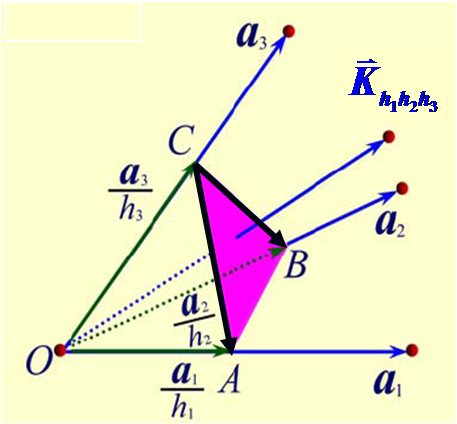
\includegraphics[height=1.65in,width=1.70in,viewport=0 0 245 224,clip]{Figures/Reciprocal_lattice_plane.png}
\caption{\small 倒格子矢量$\vec G$与\textrm{Miller}指数为$(h_1h_2h_3)$的晶面.}%(与文献\cite{EPJB33-47_2003}图1对比)
\label{Fig:Madelung_constant}
\end{figure}
\textrm{Miller}指数为$(h_1h_2h_3)$的晶面(\textcolor{magenta}{玫红色})中
\begin{displaymath}
	\bar{CA}=\dfrac{\vec a_1}{h_1}-\dfrac{\vec a_3}{h_3}\quad\bar{CB}=\dfrac{\vec a_2}{h_2}-\dfrac{\vec a_3}{h_3}
\end{displaymath}
有
\begin{displaymath}
	\begin{aligned}
		\vec G\cdot\bar{CA}=&(h_1\vec b_1+h_2\vec b_2+h_3\vec b_3)\cdot(\dfrac{\vec a_1}{h_1}-\dfrac{\vec a_3}{h_3})=\vec b_1\cdot\vec a_1-\vec b_3\vec a_3=1-1=0\\
	\vec G\cdot\bar{CB}=&(h_1\vec b_1+h_2\vec b_2+h_3\vec b_3)\cdot(\dfrac{\vec a_2}{h_2}-\dfrac{\vec a_3}{h_3})=\vec b_2\cdot\vec a_2-\vec b_3\vec a_3=1-1=0
	\end{aligned}
\end{displaymath}
因此$\vec G$与\textrm{Miller}指数为$(h_1h_2h_3)$的晶面正交\\得证

5. 证明:~两种一价离子组成的一维晶格的\textrm{Madelung}常数为$a=2ln2$

证明:~
\begin{figure}[h!]
\centering
\vspace*{-0.05in}
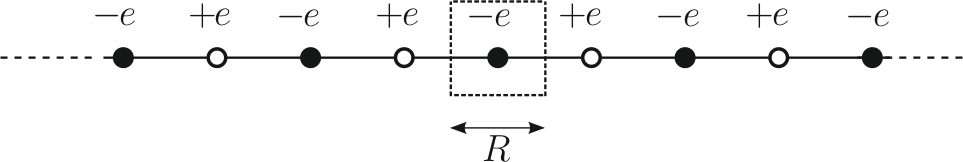
\includegraphics[height=0.65in,width=3.65in,viewport=0 0 963 162,clip]{Figures/Madelung_constant.png}
\caption{\small 两种一价离子组成的一维晶格示意图.}%(与文献\cite{EPJB33-47_2003}图1对比)
\label{Fig:Madelung_constant}
\end{figure}
一维晶格中两种一价离子间相互作用势表示为
\begin{displaymath}
	\begin{aligned}
		V(0)=&-a\dfrac{e^2}{R}\\
		=&-\dfrac{e^2}R\times2\bigg[\dfrac11-\dfrac12+\dfrac13-\dfrac14+\dfrac15-\cdots\bigg]\\
		=&2\dfrac{e^2}R\sum_{n=1}^{\infty}(-1)^n\dfrac1n\\
		=&-\dfrac{e^2}R2\ln2\\
		\therefore a=&2\ln2
	\end{aligned}
\end{displaymath}
得证

6. 一横截面积为$2~\mathrm{mm}\times2~\mathrm{mm}$的铜导线,通过的电流为$10~\mathrm{A}$,假设一个铜原子贡献一个传导电子,室温下铜的密度为$8.96~\mathrm{g/cm}^3$,用Drude模型计算:~\textcircled{1}在 $300~K$ 时电子的平均均方根速度和漂移速度 ;\textcircled{2}假设平均自由程为原子间距2.6,估计弛豫时间 ;\textcircled{3}计算铜的电导率。

解:~\textcircled{1}由经典的能量均分定理可得
\begin{displaymath}
	v_{\mathrm{rms}}=\bigg(\dfrac{3k_{\mathrm{B}}T}{m_e}\bigg)^2=\bigg[\dfrac{3\big(1.38\times10^{-23}\mathrm{J/K}\big)(300\mathrm{K})}{9.11\times10^{-31}}\mathrm{kg}\bigg]=1.17\times10^5\mathrm{m/s}
\end{displaymath} 
%由式\eqref{eq:valence_density}可得
因此传导电子密度为
\begin{displaymath}
	n=N_0\times\dfrac{Z\rho_m}{A}=6.02\times10^{23}\times\dfrac{1\times8.96}{63.5}\mathrm{cm}^{-3}=8.49\times10^{22}\mathrm{cm}^{-3}
\end{displaymath} 
由电流密度$\vec J=-nev_d$,可得电子的漂移速度
\begin{displaymath}
	v_d=\dfrac{J}{ne}=\dfrac{10\mathrm{A}}{4\times10^{-6}\mathrm{m}^2}\times\dfrac1{(8.49\times10^{28}\mathrm{m}^{-3})(1.6\times10^{-19}\mathrm{C})}=1.8\times10^{-4}\mathrm{m/s}
\end{displaymath} 
电子的漂移速度$v_d$和平均均方根速度$v_{\mathrm{rms}}$比值为
\begin{displaymath}
	v_d/v_{\mathrm{rms}}=1.5\times10^{-9}
\end{displaymath}
\textcircled{2}电子的弛豫时间为
\begin{displaymath}
	\tau=\dfrac{\mathscr{l}}{r_{\mathrm{rms}}}=\dfrac{2.6\times10^{-10}\mathrm{m}}{1.2\times10^5\mathrm{m/s}}=2.2\times10^{-15}\mathrm{s}
\end{displaymath}
%因此该模型中电子每秒完成几百万亿次碰撞。
\textcircled{3}%由式\eqref{eq:Electron_conduct} 计算得到
铜的电导率为
\begin{displaymath}
	\sigma=\dfrac{ne^2\mathscr{l}}{m_2v_{\mathrm{rms}}}=5.3\times10^6(\Omega\cdot\mathrm{m})^{-1}
\end{displaymath} 

7. 如果离子电荷加倍,会对\textrm{NaCl}晶格常数和结合能有什么影响(假定排斥势不变)

解:~根据离子晶体的相互作用势函数式\eqref{eq:SSI-03},在离子平衡位置附近,取近似
$n\mathrm{exp}(-r)\approx\dfrac1{r^n}$,并将物理常数记作$\alpha$,参数记作$C$,可有
\begin{displaymath}
	U(r)=-\dfrac{\alpha q^2}r+\dfrac{C}{r^n}
\end{displaymath}
由离子晶体平衡条件
\begin{displaymath}
	\dfrac{\mathrm{d}U}{\mathrm{d}r}\bigg|_{r_0}=\dfrac{\alpha q^2}{r_0^2}-\dfrac{nC}{r_0^{n+1}}=0
\end{displaymath}
可得参数$C$为
\begin{displaymath}
	C=\dfrac{\alpha q^2}nr_0^{n-1}	
\end{displaymath}
因此,\textrm{NaCl}的晶格常数为
\begin{displaymath}
	r_0(e)=\bigg(\dfrac{nC}{\alpha e^2}\bigg)^{\dfrac{1}{n+1}}
\end{displaymath}
所以当$q=e\rightarrow2e$时,可有
\begin{displaymath}
	r_0(2e)=\bigg(\dfrac{nC}{4\alpha e^2}\bigg)^{\dfrac{1}{n+1}}=4^{\frac{1}{n+1}}r_0(e)
\end{displaymath}
相应地,平衡位置附近的结合能
\begin{displaymath}
	U(r_0)=-\dfrac{\alpha e^2}{r_0}(1-\dfrac1n)
\end{displaymath}
因为平衡位置和电荷的变化
\begin{displaymath}
	U(2e)=-\dfrac{4\alpha e^2}{r_0(2e)}(1-\dfrac1n)=4^{\frac{n}{n+1}}U(r_0)
\end{displaymath}

8. 经过$sp^3$杂化后形成的共价键,其方向沿立方体的四条对角线,求共价键之间的夹角

解:~$sp^3$杂化形成共价键的过程如图\ref{Bond_Hybrid}的左边所示。共价键沿立方体四条对角线,与中心构成正四面体。图\ref{Bond_Hybrid}的右图中,以甲烷为例,给出$sp^3$杂化的几何关系,其中\textrm{C}原子位于正四面体中心,四个\textrm{H}原子位于正四面体顶点
\begin{figure}[h!]
\centering
\vspace{-5.5pt}
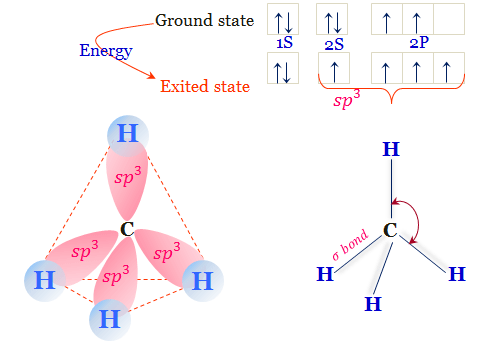
\includegraphics[height=1.75in,width=2.50in,viewport=0 0 520 370,clip]{Figures/methane-gas.png}
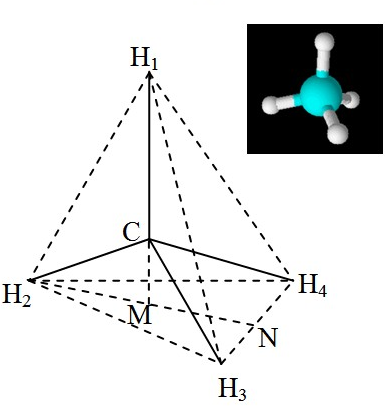
\includegraphics[height=1.75in,width=2.50in,viewport=0 0 520 370,clip]{Figures/Tetrahedron.png}
\caption{\textrm{甲烷中的C原子轨道$sp^3$杂化和键角计算示意图}}
\label{Bond_Hybrid}
\end{figure}
设正四面体\textrm{H1-H2-H3-H4}的棱长为$a$,\textrm{C-H1}延长线与\textrm{H2-H3-H4}平面交于\textrm{M}点,\textrm{M}点为等边$\vartriangle$\textrm{H2-H3-H4}的中心,可有%\textrm{C-H}键的键长
\begin{displaymath}
	\overbar{\mathrm{MH}}_i=\dfrac{a}2/\cos{30^{\circ}}=\dfrac{\sqrt 3a}3\quad i=2,3,4
\end{displaymath}
据勾股定理可有
\begin{displaymath}
	\overbar{\mathrm{MH}}_1=\sqrt{a^2-\frac{a^2}3}=\sqrt{\frac23}a
\end{displaymath}
设\textrm{C-H}键的键长为$x$,则在直角$\vartriangle$\textrm{M-C-H3}中,利用勾股定理可有
\begin{displaymath}
	\begin{aligned}
	\dfrac{a^2}3+\bigg(\sqrt{\frac23}a-x\bigg)^2=&x^2\\
	\therefore~x=&\sqrt{\frac38}a
	\end{aligned}
\end{displaymath}

$\therefore$~等腰$\bigtriangleup$\textrm{C-H1-H2}中,三边长依次为${\sqrt \dfrac38}a$,$\sqrt{\dfrac38}a$,$a$,由余弦定理,可有
\begin{displaymath}
	\cos\angle\mathrm{H1CH2}=\dfrac{2\times\dfrac38a^2-a^2}{2\times\dfrac38a^2}=-1/3
\end{displaymath}
即共价键$\angle\mathrm{HCH}=109^{\circ}28^{\prime}$

9.~写出一维近自由电子近似下第$n$个能带$(n=1,2,3)$中,简约波矢$k=\dfrac{\pi}{2a}$的0级波函数

解:~根据一维近自由电子0级波函数表达式
\begin{displaymath}
	\Psi_k(x)=\dfrac1{\sqrt L}\mathrm{e}^{\mathrm{i}kx}=\dfrac1{\sqrt L}\mathrm{e}^{\mathrm{i}\bar{k}x}\mathrm{e}^{\mathrm{i}\frac{2\pi}amx}=\dfrac1{\sqrt L}\mathrm{e}^{\mathrm{i}\frac{\pi}{2a}x}\cdot\mathrm{e}^{\mathrm{i}\frac{2\pi}amx}=\dfrac1{\sqrt L}\mathrm{e}^{\mathrm{i}\frac{2\pi}a(m+\frac14)x}
\end{displaymath}
可以知道:
\begin{itemize}
	\item 第一能带:~$m\cdot\frac{2\pi}{a}=0$,$m=0$,有$\Psi_k(x)=\dfrac1{\sqrt L}\mathrm{e}^{\mathrm{i}\frac{\pi}{2a}x}$
	\item 第二能带:~$m\cdot\frac{2\pi}{a}=-\frac{2\pi}{a}$,$m=-1$,有$\Psi_k(x)=\dfrac1{\sqrt L}\mathrm{e}^{\mathrm{i}\frac{\pi}{2a}x}\cdot\mathrm{e}^{\mathrm{i}\frac{-2\pi}{a}x}=\dfrac1{\sqrt L}\mathrm{e}^{-\mathrm{i}\frac{3\pi}{2a}x}$
	\item 第三能带:~$m\cdot\frac{2\pi}{a}=\frac{2\pi}{a}$,$m=1$,有$\Psi_k(x)=\dfrac1{\sqrt L}\mathrm{e}^{\mathrm{i}\frac{\pi}{2a}x}\cdot\mathrm{e}^{\mathrm{i}\frac{2\pi}{a}x}=\dfrac1{\sqrt L}\mathrm{e}^{\mathrm{i}\frac{5\pi}{2a}x}$
\end{itemize}

10.~用$|n\rangle$表示一维晶格的第$n$个格点的$s$态,在只计入最近邻作用的紧束缚近似下,写出矩阵元$\langle m|H|n\rangle$的表达式
解:~对于由$N$个相同原子组成的一维晶格,第$n$个格点的原子位移矢量为$\vec x_n$\\
作为孤立原子,势函数表示为$u(\vec r-\vec x_n)$,相应的$s$态波函数$\phi_s(\vec r-\vec x_n)$,能量为$E^{(0)}$\\
在晶格中$s$电子感受到的势函数为$v(\vec r)$,紧束缚近似下,电子具有$N$重简并。考虑微扰后,0级近似的波函数记作
\begin{displaymath}
	\Psi_k(\vec r)=\sum_nC_{n\vec k}\phi(\vec r-\vec x_n)
\end{displaymath}
这里$C_{n\vec k}$是与$n\vec k$有关的函数。根据\textrm{Bloch}定理,波函数写成
\begin{displaymath}
	\begin{aligned}
		\Psi_k(\vec r)=&\mathrm{e}^{\mathrm{i}\vec k\cdot\vec r}\sum_n\mathrm{e}^{-\mathrm{i}\vec k\cdot(\vec r-\vec x_n)}\phi(\vec r-\vec x_n)=\sum_n\mathrm{e}^{\mathrm{i}\vec k\cdot\vec x_n}\phi(\vec r-\vec x_n)\\
		\therefore~C_{n\vec k}=&\mathrm{e}^{\mathrm{i}\vec k\cdot\vec x_n}
	\end{aligned}
\end{displaymath}

对\textrm{Schr\"odinger}方程
\begin{displaymath}
	H\Psi_k(\vec r-\vec x_n)=E\Psi_k(\vec r)
\end{displaymath}
作一阶微扰,$H$可以取为
\begin{displaymath}
	H=-\dfrac{\hbar^2\nabla^2}{2m}+v(\vec r)=\bigg[-\dfrac{\hbar^2\nabla^2}{2m}+u(\vec r-\vec x_n)\bigg]+[v(\vec r)-u(\vec r-\vec x_n)]=H_0+H^{\prime}
\end{displaymath}
其中$H^{\prime}=v(\vec r)-u(\vec r-\vec x_n)$是微扰项。在$\vec x_n$附近$H^{\prime}$非常小,而离$\vec x_n$较远处,要求$\phi(\vec r-\vec x_n)$趋于0

因此微扰后能量取一级近似,可以写成
\begin{displaymath}
	E=\dfrac{\int\Psi_k^{\ast}(\vec r)H\Psi_k(\vec r)\mathrm{d}\vec r}{\int\Psi_k^{\ast}(\vec r)\Psi_k(\vec r)\mathrm{d}\vec r}
\end{displaymath}
因此所求的矩阵元
\begin{displaymath}
	\begin{aligned}
		\langle m|H|n\rangle=&\int\Psi_k^{\ast}(\vec r)H\Psi_k(\vec r)\mathrm{d}\vec r\\
		=&\int\Psi_k^{\ast}(\vec r)\big(H_0+H^{\prime}\big)\Psi_k(\vec r)\mathrm{d}\vec r\\
		=&\int\Psi_k^{\ast}(\vec r)\sum_n\big(H_0+H^{\prime}\big)\mathrm{e}^{\mathrm{i}\vec k\cdot\vec x_n}\phi(\vec r-\vec x_n)\mathrm{d}\vec r\\
		=&E^{(0)}\int\Psi_k^{\ast}(\vec r)\Psi_k(\vec r)\mathrm{d}\vec r+\int\sum_m\mathrm{e}^{\mathrm{i}\vec k\cdot\vec x_m}\phi^{\ast}(\vec r-\vec x_m)\sum_nH^{\prime}\mathrm{e}^{\mathrm{i}\vec k\cdot\vec x_n}\phi(\vec r-\vec x_n)\mathrm{d}\vec r\\
		=&NE^{(0)}+\sum_m\sum_n\mathrm{e}^{\mathrm{i}\vec k\cdot(\vec x_n-\vec x_m)}\int\phi^{\ast}(\vec r-\vec x_m)H^{\prime}\phi(\vec r-\vec x_n)\mathrm{d}\vec r\\
		=&NE^{(0)}+N\sum_n\mathrm{e}^{\mathrm{i}\vec k\cdot(\vec x_n-\vec x_m)}\int\phi^{\ast}(\vec r-\vec x_m)H^{\prime}\phi(\vec r-\vec x_n)\mathrm{d}\vec r
	\end{aligned}
\end{displaymath}



{\heiti 第十二章~习题}

1.~简单说明密度泛函理论和\textrm{Kohn-Sham}方程中的交换-相关势与交换-相关泛函的关系

{\heiti 回答要点:}\\
(1)密度泛函理论的核心:~体系的基态性质完全可以由体系的基态密度确定,体系的基态能量泛函在体系基态密度取变分极小值\\
(2)密度泛函理论将体系的基本变量由波函数转换为密体,描述问题的变量由$3N$维将为$3$维,大大简化了求解难度\\
(3)体系基态能量的密度泛函的精确形式未知,\textrm{Kohn-Sham}引入无相互作用粒子体系,将真实体系与无相互作用体系的差别放入交换-相关泛函中\\
(4)\textrm{Kohn-Sham}方程形式上是单粒子函数的运动方程,它把波函数重新引入作为获得体系基态密度的重要工具(中间桥梁)\\
(5)\textrm{Kohn-Sham}方程中的交换-相关势源自交换-相关能泛函:~$V_{\mathrm{XC}}=\dfrac{\delta E_{\mathrm{XC}}[\rho]}{\delta\rho(\vec r)}$,交换-相关势出现在\textrm{Kohn-Sham}方程中,交换-相关能则用于体系基态总能量的计算

2.~简单说明交换-相关泛函的分类方式

{\heiti 回答要点:}\\
(1)局域(自旋)密度近似\textrm{(L(S)DA)}:~最简单的交换-相关泛函形式,泛函仅与电荷密度$\rho(\vec r)$的空间分布有关(如果是\textrm{LSDA}要考虑电子自旋的影响)\\
(2)广义梯度近似\textrm{(GGA):~}交换-相关泛函与电荷密度$\rho(\vec r)$的空间分布及其空间梯度$\nabla\rho(\vec r)$有关,当电荷密度变化剧烈时,\textrm{GGA}比\textrm{L(S)DA接近真实情况}\\
(3)动态广义梯度近似\textrm{(meta-GGA)}:~在\textrm{GGA}基础上考虑密度空间分布的两阶梯度$\nabla^2\rho(\vec r)$对泛函的贡献\\
(4)杂化泛函\textrm{(hybrid-XC)}:~针对密度泛函理论将连续变量密度代替离散变量粒子引入的误差,引入部分\textrm{Hartree-Fock}方法中精确交换作用的贡献,与经典交换泛函杂糅(通过系数调节),得到更高精度的泛函。杂化泛函的计算量一般比较巨大,目前主要大量用于化学分子、化学反应等高精度计算中,周期体系计算中应用较少

3.~简单说明赝势的构造原则,可分离赝势引入的原因及应用意义

{\heiti 回答要点:}\\
(1)赝势的构造原则:~兼顾``柔软性''(展开的平面波数目尽可能少)和``可移植性''(使用的范围尽可能的广泛)。这两个原则是彼此矛盾的,实际构造赝势的时候,需要根据需求有针对性地进行优化
(2)第一原理势的构造通过设计赝波函数,逆向求解原子径向方程,获得局域的赝势(仅限于径向部分)\\
(3)考虑角度部分贡献后的赝势只是半局域\textrm{(semi-local)}的,与角动量量子数$l$和磁量子数$m$有关,这样的赝势在计算中应用非常不方便\\
(4)将赝波函数中包含角度部分并引入近似实现角动量量子数$l$和磁量子数$m$的变量分离,可以获得完全局域的赝势,非局域部分贡献则通过近似后的赝波函数构造投影函数得到\\
(5)通过投影函数实现赝势的局域-非局域分离,可以在计算软件中实现赝势的快速构造,大大提升计算效率。但也因此引入计算误差的产生,可以通过扩大变分空间克服

4.~简要说明\textrm{PAW}方法中的``全电子''计算与\textrm{LAPW}方法中的``全势''计算的联系与区别

{\heiti 回答要点:}\\
(1)\textrm{PAW}方法中的``全电子''计算强调计算过程中保留了电子波函数在靠近原子核附近的振荡行为,突出对赝势方法的赝波函数部分的改进\\
(2)\textrm{LAPW}方法中的``全势''突出电子在整个空间感受到的势与真实情况相近,突出的是对赝势方法中赝势部分的改进\\
(3)势函数决定电子波函数的行为,从计算精度上说,全势方法的精确程度会更高一点,但计算量也更大\\
(4)两种方法都是在赝势-平面波方法基础上发展起来的,但由于采用了不同的实现路线,所以选择了两个不同的词本质上对同一个问题不同侧面予以强调,核心目标都是为了提高计算电子体系的精度

5.~简单说明电子相关对计算的影响\\

{\heiti 回答要点:}\\
(1)由于用联系的粒子密度代替不连续的粒子,密度泛函方法先天就存在对粒子相关问题考虑的不足
(2)对于含有$d$、$f$电子等局域电子体系,电子相关问题对计算影响更显著,甚至会定性错误,所以对这些体系应用密度泛函方法计算一定要注意
(3)电子相关问题可以通过引入多粒子相关函数予以克服,最常用的包括\textrm{Green~Function}方法,化学家也有应用\textrm{CI(Configuration Interaction)}方法,但计算量增加的非常可观
(4)电子相关主要影响的是体系的某些物理性质,如果只和体系总能有关的物理性质(如基态体积、体弹模量等),受电子相关的影响很小
